This search~\cite{CMS:2016nhb} looks for evidence of SUSY in events with particles identified as top quarks. An excess of events containing top-tagged jets (top tags) over the~\sm~background may be evidence of the production of top squark pairs, whose existence has been motivated as a solution to the hierarchy problem (Section \ref{sec:problems}).  The possibility of top squarks in mass range below about 450 GeV has largely been ruled out by results from other experiments.  However, considerations of naturalness implore us to look for top squarks nonetheless. The analysis is optimized to be sensitive to signatures resembling the simplified models shown in Fig. \ref{fig:hadstopSMS}.
\begin{figure}[h]
\centering
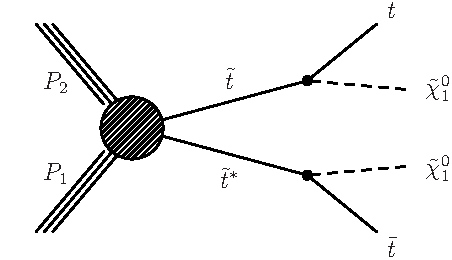
\includegraphics[width=0.45\textwidth]{figures/SusySearches/HadStop2015/T2tt.pdf}
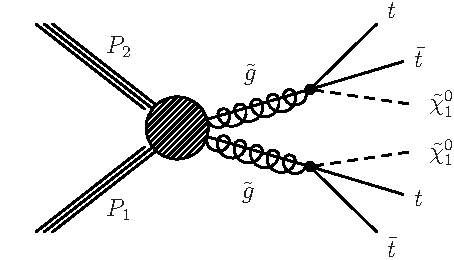
\includegraphics[width=0.45\textwidth]{figures/SusySearches/HadStop2015/T1tttt.pdf}\\
\caption{
  The simplified models used for the optimization and interpretation of the hadronic search for SUSY in events with top-tagged jets.
  They are T2tt (left) and T1tttt (right).
}
\label{fig:hadstopSMS}
\end{figure}


In addition to the multiplicity of top-tagged jets, other observables are used for signal/background discrimination, including the $\Ht$, $\met$, $\njets$, $\nbjets$, and the stransverse mass $M_{\text{T2}}$~\cite{Lester:1999tx}. Top-tagged jets are constructed by considering all three-jet combinations in an event, and selecting a combination with an invariant mass consistent with the top quark mass. After identifying this top-tagged jet, the remaining jets in the event are analyzed and checked for consistency with a second top quark in the event, inferred by the presence of a b-tagged jet. In the event that both systems (the top-tagged system and the remnant b-tagged jet) are reconstructed, the $M_{\text{T2}}$ is computed taking the four-vectors of the two systems as input, along with the $\met$ of the event. 

Events are collected using the hadronic trigger discussed in Section \ref{sec:anatrig}. The probability for the trigger to fire on an event that passes the baseline selection is greater than 98\%. The full baseline selection if defined as follows. Events are accepted if they have
\begin{itemize}
\item no reconstructed, isolated lepton with a $\pt>10$ GeV and $|\eta|<2.4$;
\item no reconstructed, isolated particle track with a $\pt>10$ GeV and $|\eta|<2.4$;
\item $\Ht>500$ GeV;
\item $\met>200$ GeV;
\item an azimuthal separation between the $\mht$ and the leading three jets $\Delta\phi(\mht$, jet$_{1,2,3})>$ 0.5, 0.5, 0.3;
\item $N_t\geq1$, where $N_t$ is the top-tag multiplicity;
\item $\nbjets\geq1$, and
\item $M_{\text{T2}}>200$ GeV.
\end{itemize}
After the baseline selection, events are further subdivided into search bins defined by rectangular boundaries in the dimensions of $\met$, $M_{\text{T2}}$, $\nbjets$, and $N_t$. 
%%%%%%%%%%%%%%%%%%%%%%%%%%%%%%%%%%%%%%%%%%%%%%%%%%

%-------------
The most significant background across the search regions comes from the SM $\ttbar$ production or W-boson production, where either ${\rm W}\rightarrow \ell\nu$ and the lepton ($\ell={\rm e},\mu$) is not detected or ${\rm W}\rightarrow \tau\nu$ and the $\tau$ lepton decays hadronically. Generally, the next largest contribution comes from $\zinv$ production in association with jets (including heavy-flavour jets) in which the neutrino pair gives large \MET and the top quark conditions are satisfied by an accidental combination of the jets. The QCD multi-jet contribution and the contribution from other rare SM processes are subdominant across all bins. The largest rare SM process contribution (though still small) comes from $\ttbar$-Z with the Z boson decaying into a pair of neutrinos.  


\subsubsection{Systematic uncertainty in $\zinv$ prediction}
An overall simulation-to-data normalization factor is derived in a control region with 0 b-tagged jets and applied to the $\zinv$ simulation as part of the final prediction. A comparison of the normalization factor derived from the dielectron sample with that derived from the dimuon sample is shown in Fig. \ref{fig:ZInvNorm}.
\begin{figure}[tb!]
\centering
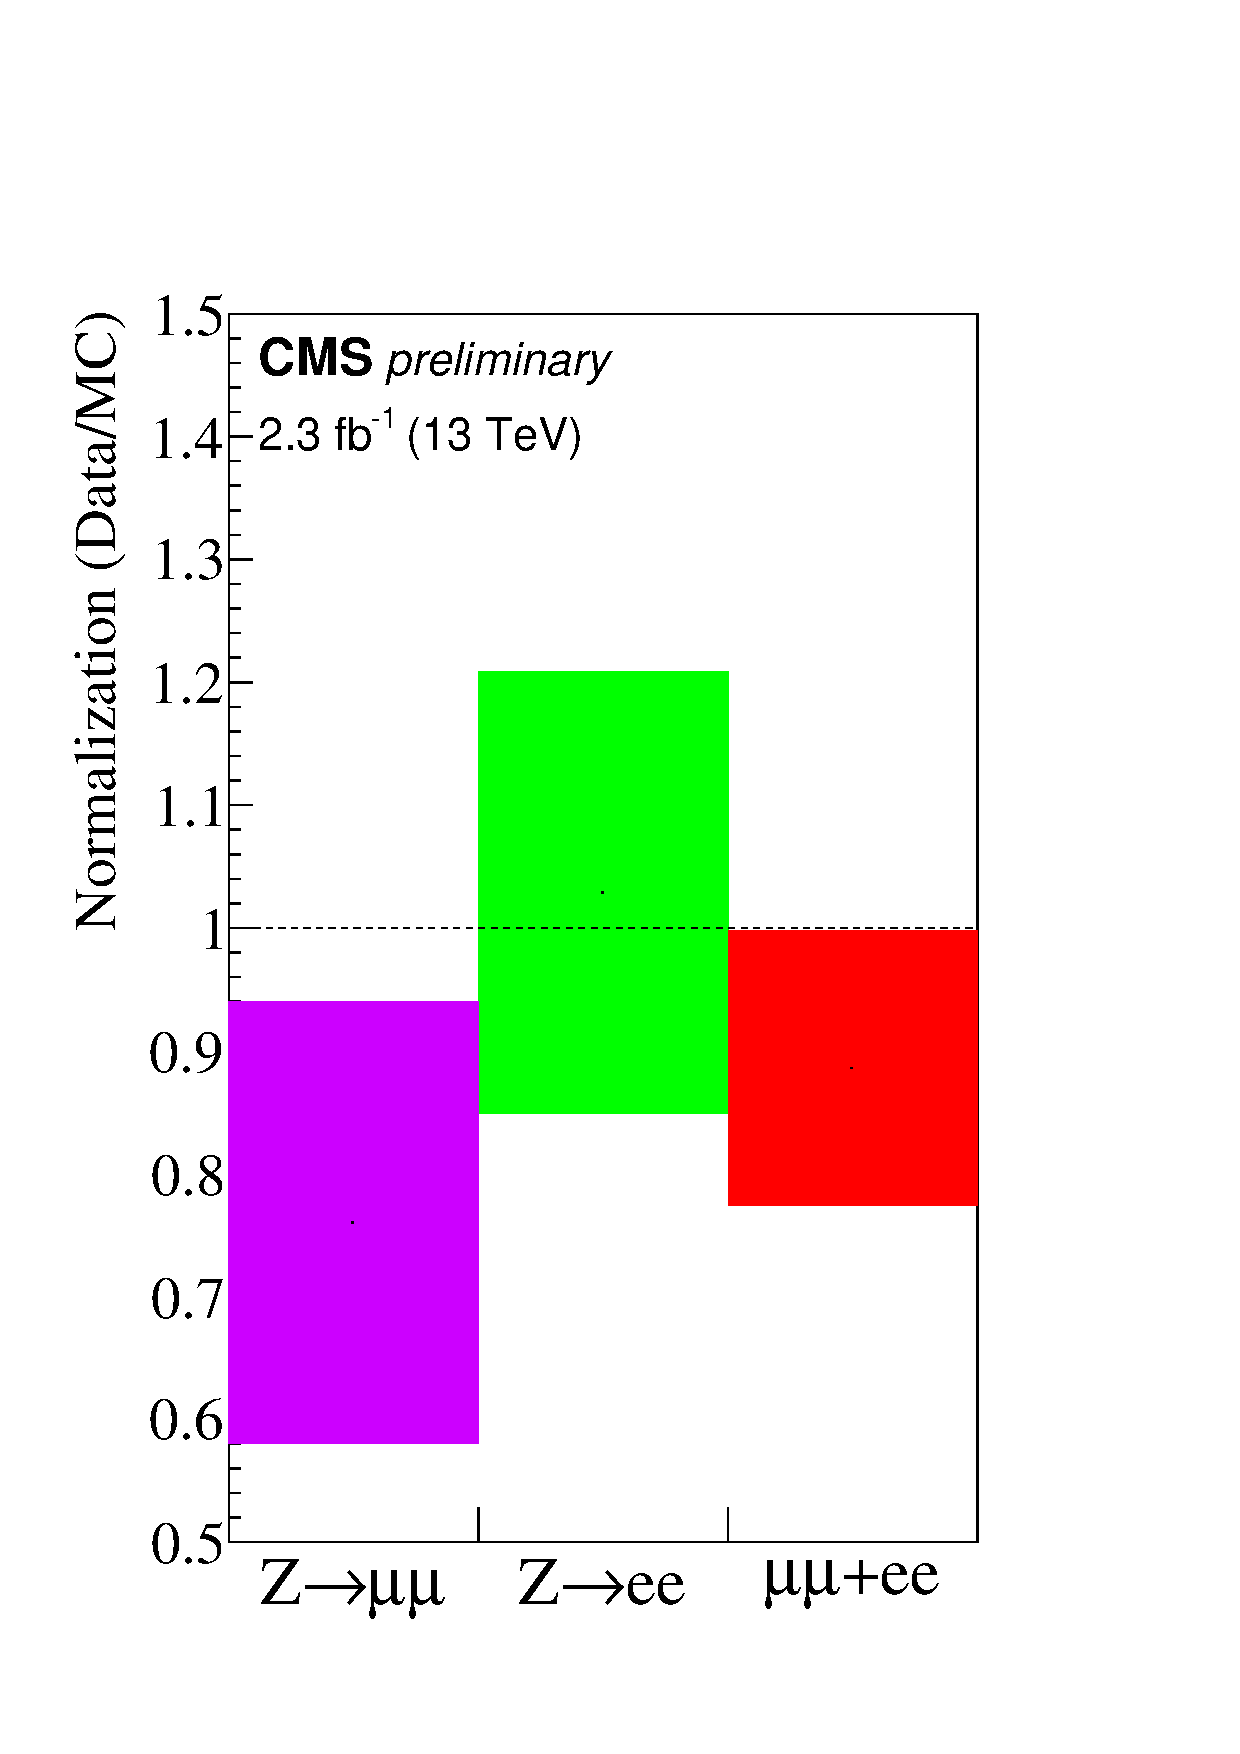
\includegraphics[width=0.4\linewidth]{figures/SusySearches/HadStop2015/NormFactors.pdf}
\caption{The data-simulation normalization factor computed from the dimuon sample (magenta), the dielectron sample (green), and the combined dielectron $+$ dimuon sample (red). }
\label{fig:ZInvNorm}
\end{figure}
\noindent
The electron- and muon-derived normalization factors agree within statistical uncertainties, indicating that a trivial combination of the electron and muon data is justifiable in the derivation of the normalization factor and its uncertainty. This reduces the systematic uncertainty in the $\zinv$ prediction associated with the normalization by approximately 30\%. An interpretation of these results in terms of a simplified model involving top squark production is given in the 2015 results section (Section \ref{sec:2015results}).

\subsubsection{Systematic uncertainties}

The predicted number of SM background events and the number of events observed in data for each of the search regions are shown in Figure~\ref{fig:baseline_SR} and Tabulated in Ref.~\cite{CMS:2016nhb}. 

%%%%%%%%%%%%%%%%%%%%%%%%%%%%%%%%%%%%%%%%%%%%%%%%%%
\begin{figure}[htbp]
  \begin{center}
  \begin{tabular}{cc}
\hspace{-1.5cm}
  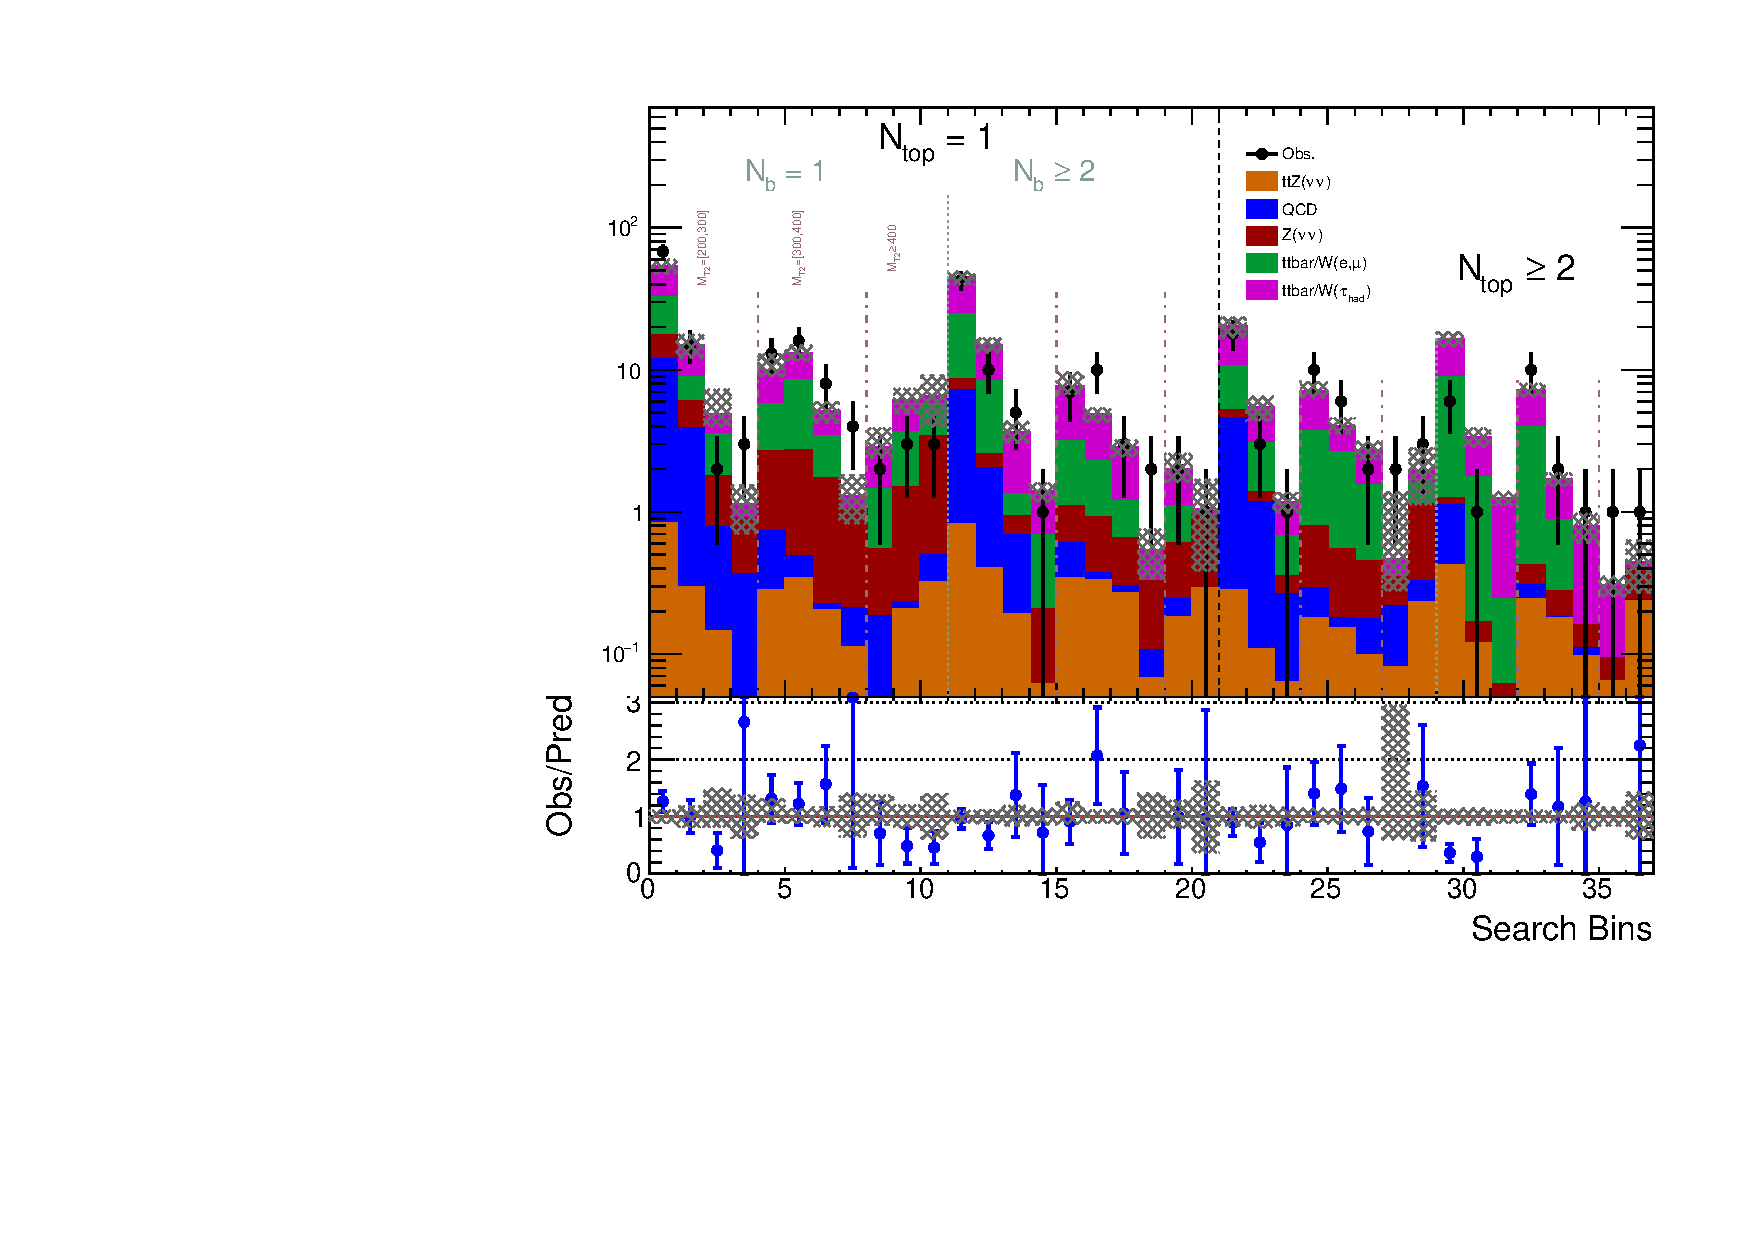
\includegraphics[width=0.85\textwidth]{figures/SusySearches/HadStop2015/UnblindPlots.pdf}
  \end{tabular}
  \caption{Data are shown as black points. The total predictions are shown in filled solid area. The bottom plot shows the ratio of data over total background prediction in each search bin. Only statistical uncertainties are propagated to the ratio. The numbering scheme is given in Ref. \cite{CMS:2016nhb}.}
    \label{fig:baseline_SR}
  \end{center}
\end{figure}
Good agreement is observed between the SM background predictions and the yields observed in data for each search bin, within uncertainties.

%The following uncertainties on the signal modeling are taken into account when the limits are determined: simulation sample size, luminosity determination ($4.6\%$), lepton and isolated track veto, b-tag efficiency corrections used to scale simulation to data, trigger efficiency, QCD renormalisation and factorization scales, initial/final state radiation (ISR/FSR), signal acceptance and efficiency arising from the jet energy-momentum corrections, jet energy-momentum resolutions, and propagated to \MET, parton distribution functions (PDF) of the proton

The results are interpreted in terms of the simplified model scenarios shown in Fig. \ref{fig:hadstopSMS} using a similar limit setting technique discussed in Section \ref{sec:ra2b2015}. Uncertainties considered are similar to those discussed in Section \ref{sec:ra2b2015}, in addition to uncertainties associated with differences in the top-quark tagging efficiency and false positive rate between the CMS fast and full simulations, on the order of a few percent.

%%%%%%%%%%%%%%%%%%%%%%%%%%%%%%%%%%%%%%%%%%%%%%%%%%

%-------------
The observed cross section upper limits on signal models of direct top squark pair production, T2tt and T1tttt, are shown in Figure~\ref{fig:fulllimit_T2tt_T1tttt}, together with contours that correspond to points for which the observed (black contour) and expected (red-dashed contour) upper limits equal the theoretical signal cross sections.
%%%%%%%%%%%%%%%%%%%%%%%%%%%%%%%%%%%%%%%%%%%%%%%%%%
\begin{figure}[htbp]
  \begin{center}
  \begin{tabular}{cc}
\hspace{-1.5cm}
  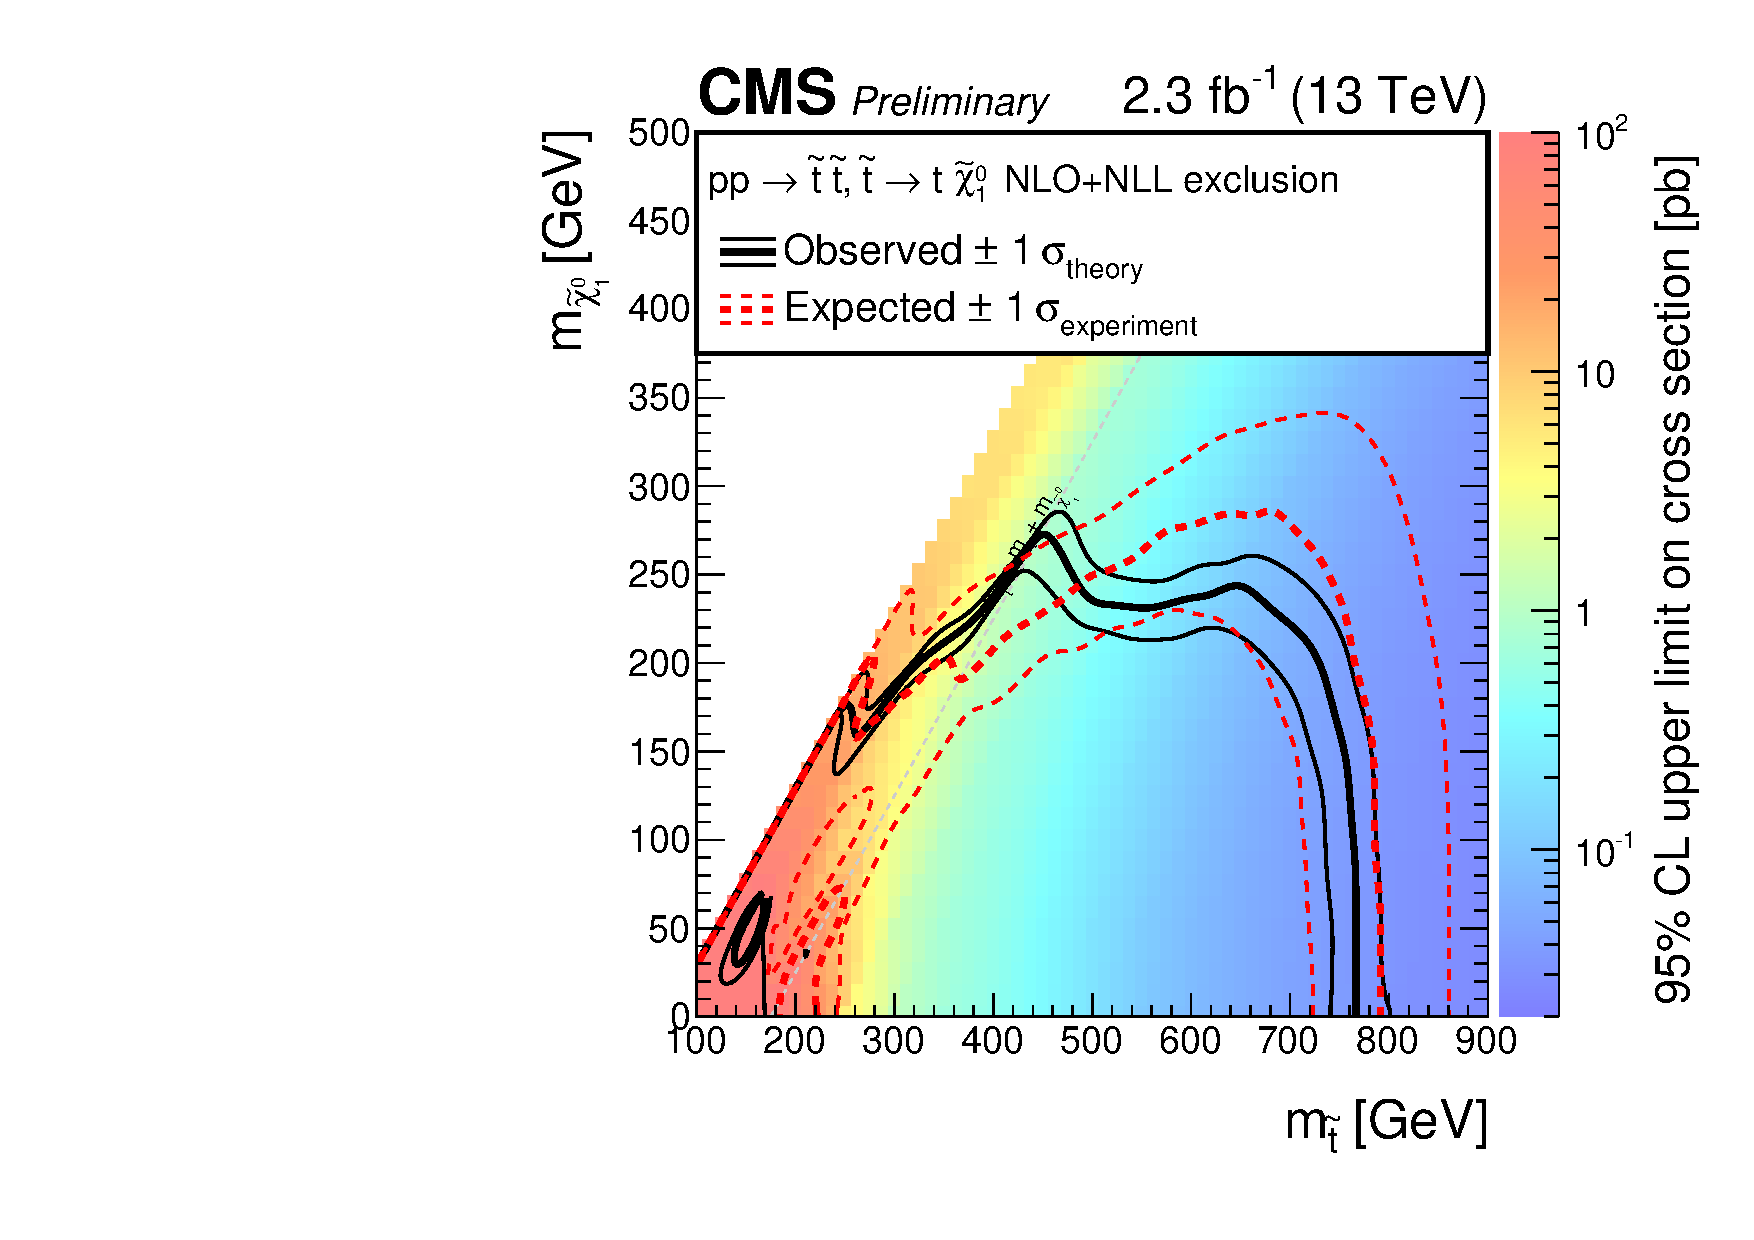
\includegraphics[angle=0,width=0.48\textwidth]{figures/SusySearches/HadStop2015/BR_1p00_Stop_OnlyXSEC.pdf}
  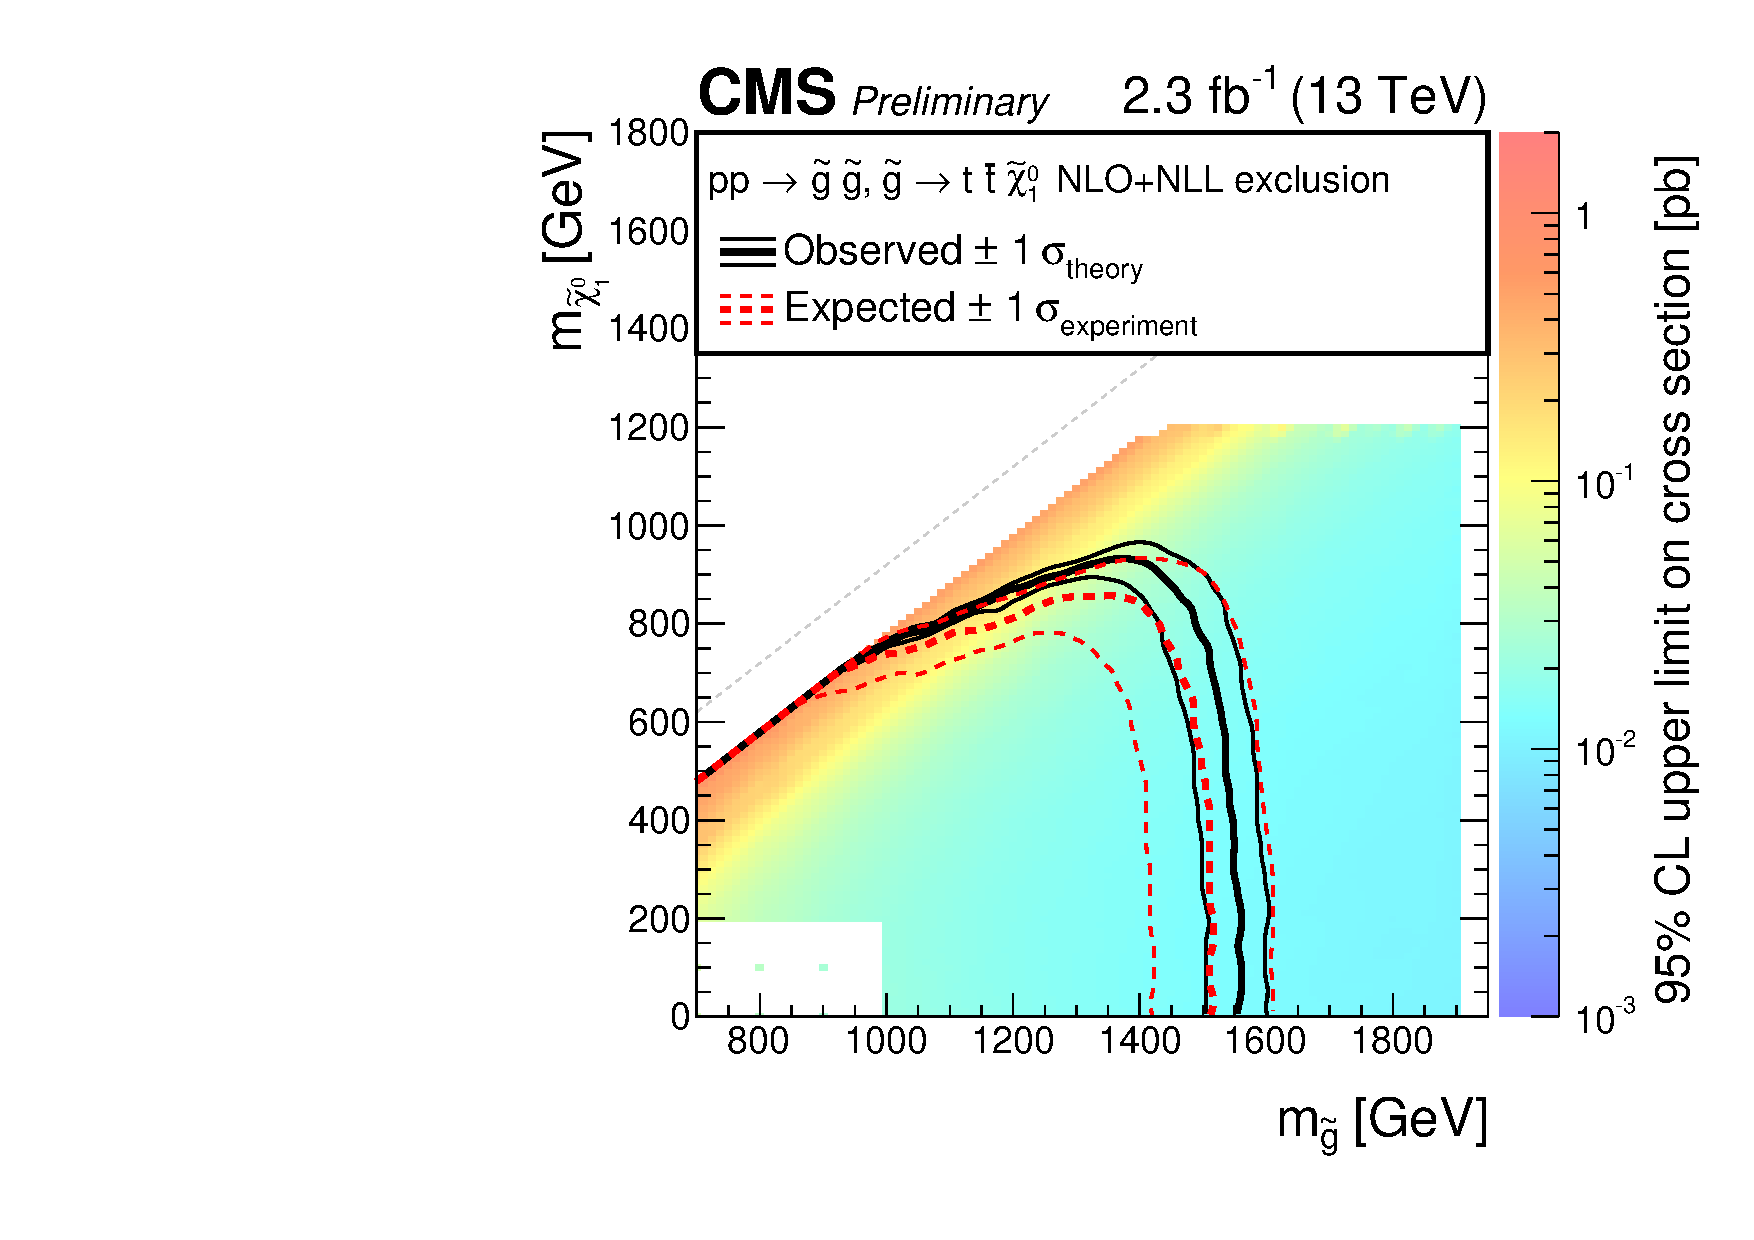
\includegraphics[angle=0,width=0.48\textwidth]{figures/SusySearches/HadStop2015/zinv_improvement_BR_1p00_Gluino_OnlyXSEC.pdf}
  \end{tabular}
  \caption{Expected and observed limits. The left shows the limits on the T2tt model, where the branching ratio for the top squark to decay to a top quark and neutralino is 100\%. The right plots shows the limits on the T1tttt model, where the branching ratio for a top squark to decay to a top quark and neutralino is 50\%. The $\zinv$ prediction derived from the combined dimuon and dielectron control samples, as described in Section \ref{sec:zinv}, are used.}
    \label{fig:fulllimit_T2tt_T1tttt}
  \end{center}
\end{figure}
%%%%%%%%%%%%%%%%%%%%%%%%%%%%%%%%%%%%%%%%%%%%%%%%%%

%
The expected exclusion curves show the cases in which the background uncertainties are varied by one standard deviation.

In the T2tt model, shown in the left plot of Fig.~\ref{fig:fulllimit_T2tt_T1tttt}, where both top squarks decay to top quarks and neutralinos, the median expected lower limit on the top squark mass reaches 790~\GeV~, for small neutralino masses, and the observed limit excludes top squark masses below about 760~\GeV~ at 95\% confidence level.  For large neutralino masses in the same model, the median expected lower mass limit on the neutralino reaches about 280~\GeV~ with an observed limit near 220~\GeV, for a top squark mass near 650~\GeV. 
